\chapter{Background}\label{ch:background}

This chapter describes the fundamental background in different fields that is needed to understand the content of the thesis. An introduction to edge computing is presented in \cref{sec:edge_computing}. In \cref{sec:object_detection}, the \gls{dnn} approach to detect objects in the image is introduced. Finally, the frameworks and software tools used for the implementation of the thesis are introduced in \cref{sec:frameworks_and_tools}.

% ------------------------------------------------
\section{Edge Computing}\label{sec:edge_computing}
% ------------------------------------------------

Edge computing as an evolution of cloud computing brings the application hosting from centralized data centers down to the network edge, closer to the consumers and the data generated by applications, in order to reduce the latency and improve the bandwidth efficiency \cite{Kekki2018}. An illustration of the relation among cloud, edge, and end devices is shown in \cref{fig:mec}

% Figure for edge computing
\begin{figure}
    \centering
    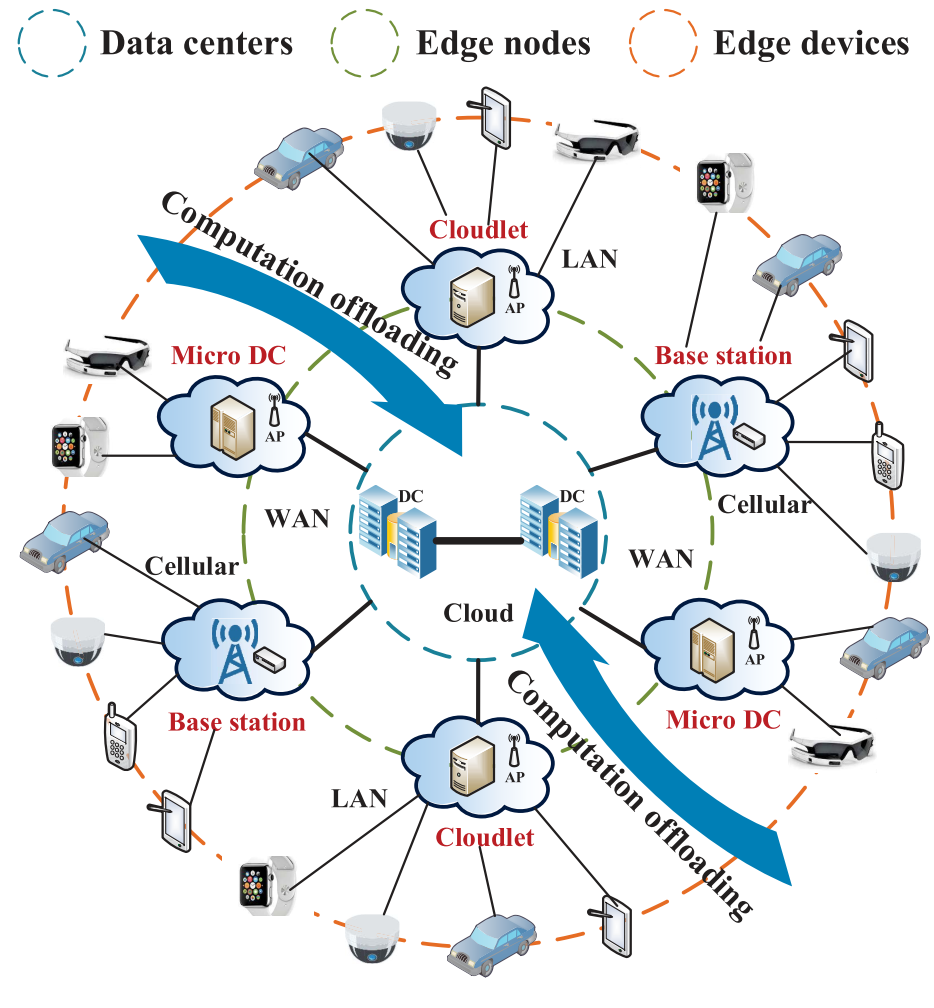
\includegraphics[width=0.6\linewidth]{figures/background/mec.png}
    \caption[A typical three-tier architecture of edge computing with the flow of computation offloading]{A typical three-tier architecture of edge computing with the flow of computation offloading \cite{Lin2019}}
    \label{fig:mec}
\end{figure}

\subsection{Development of edge computing}

Over the last two decades, cloud computing starts to its power in industry, business, and daily life by leveraging powerful infrastructures, such as remote data centers, to augment the computation capabilities of less powerful devices \cite{Lin2019}. Especially with the booming of mobile devices, e.g., smartphones, \gls{mcc}, as the integration of cloud computing and mobile computing, has become recognized as the new generation of computing. However, cloud computing cannot satisfy the latency requirements for time-sensitive tasks. As a result, many efforts have gone into reducing the latency by placing the computing units closer to the end devices. 

To leverage the \gls{wan} delays, jitters, congestion, and failures, \citeauthor*{Satyanarayanan2009} \cite{Satyanarayanan2009} first used \glspl{vm} to instantiate customized service on a nearby "cloudlet", which is a resource-abundant computer or cluster of computers placed at the edge of the Internet as a proof of concept for edge computing. Later on, \citeauthor*{Bonomi2012} \cite{Bonomi2012} introduced fog computing, which allows the end devices to use both edge and cloud computing and defines the connection between the end devices, the edge, and the cloud. In recent years, as an effort to standardize edge computing, ETSI \cite{Kekki2018} announced the \gls{mec} focusing on integrating edge computing with \gls{ran}, especially with 5G network. On the other hand, various companies, including Intel, founded the OpenFog Consortium and introduced the OpenFog as an open architectural framework for fog computing. Then, as a reconciliation of the two standards, ETSI and OpenFog consortium start to collaborate on the application of edge and fog computing. Another approach is the \gls{tsn} \cite{Satka2023}. With a focus on reducing network latency and jitters, \gls{tsn} was initially proposed as a standard for wired communication. However, in recent years, researchers have also gone into the \gls{tsn}-5G integration to achieve \glspl{kpi} in network latency and jitters. 

In the industrial domain, \glspl{iot} supported by Industrial 4.0 have been a key enabler for industrial automation. Therefore, Intel published the edge infrastructure handbook providing ready-to-deploy time-sensitive solutions for \gls{iot} applications \cite{intel-edge-2021}. 

\subsection{Edge robotics}

Robots run different algorithms on their onboard system, such as perception, \gls{slam}, navigation, and path planning. However, the robotic onboard resources are usually limited due to cost and spatial reasons. Offloading some of the computation to the edge can alleviate the workload of the robot's onboard system. This approach, sometimes also called edge robotics, is an ideal use case for edge computing. 

Many works have already proven the concept of edge robotics. \citeauthor*{Huang2022} \cite{Huang2022} show that using edge in multi-robot \gls{slam} algorithm reduces the processing latency. \citeauthor*{Sossalla2022} \cite{Sossalla2022} took a step further by offloading navigation, \gls{slam}, and control functionalities to the edge and ensured the network latency and throughput requirements by using a 5G connection. \citeauthor*{Xie2021} \cite{Xie2021} achieved real-time instance segmentation for mobile robots with limited onboard resources. In the works of \citeauthor*{Fu2019} \cite{Fu2019} and \citeauthor*{Tanwani} \cite{Tanwani}, they both show that offloading the object recognition tasks reduces the execution latency and improves the task performance. 

Although edge computation offloading in robotics does show promising results in reducing execution latency and improving task performance, \citeauthor{Saeik2021} \cite{Saeik2021} pointed out that the dynamic network conditions and the resource allocation are still open challenges in edge robotics. This left several open questions of application partitioning, offloading decision-making, and distributed task execution. 

% ----------------------------------------------------
\section{Object Detection}\label{sec:object_detection}
% ----------------------------------------------------

Object detection, as an essential part of robotic vision, is one of the algorithms the robot runs on its onboard system. It provides bounding boxes and classification of potential objects in the robot's view. In the last two decades, object detection has undergone a paradigm shift from statistical classifiers using hand-crafted features to \gls{dnn} using general-purpose learning procedures and large datasets \cite{RuizdelSolar2018}. \gls{dl}-based methods not only improve the performance of object detection but also increase the computation workload of the robotic system, making it harder to achieve real-time object detection on the robot with complex \gls{dnn} models. Therefore, edge robotics, as a method to alleviate the computation workload of the robot's onboard system, can help achieve real-time execution. 

\subsection{DNN-based object detection}

% short introduction of object detection using neural network
State-of-the-art object detection methods usually consist of a backbone, a neck, and a head, as shown in \cref{fig:object_detector}. The backbone is usually made up of pre-trained \gls{cnn} layers that are used for feature extraction, such as VGG16 \cite{Simonyan2015} and ResNet-50 \cite{He2016}. The neck usually consists of some layers used to collect feature maps from different stages. Finally, the head is responsible for predicting bounding boxes and classes of objects. 

% Figure for object detection algorithm architecture
\begin{figure}
    \centering
    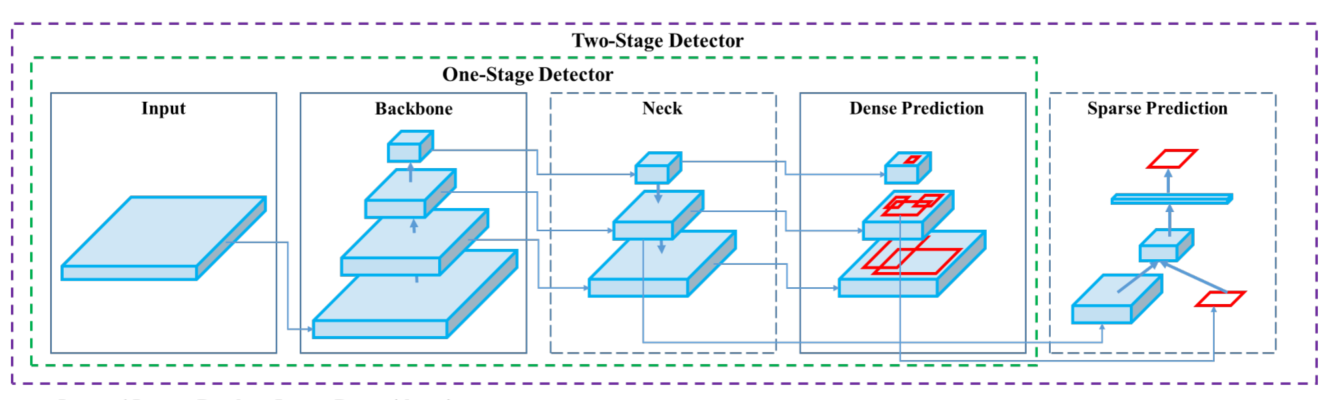
\includegraphics[width=\linewidth]{figures/background/object_detector.png}
    \caption[Architecture of object detection algorithms]{Architecture of object detection algorithms \cite{Bochkovskiy2020}}
    \label{fig:object_detector}
\end{figure}

As shown in \cref{fig:object_detector}, the object detection algorithms can be divided into two categories based on the structure of the head: one-stage detector and two-stage detector. Two-stage detectors, such as Faster R-CNN \cite{Ren2015} and Mask-RCNN \cite{He2017}, have a \gls{rpn} that generates proposals for \gls{roi}. Then, the regressor and classifier detect a bounding box and a class for that \gls{roi}. On the other hand, one-stage detectors, such as SSD \cite{Liu2016} and YOLO \cite{Redmon2016}, have only one network to do both. Benefiting from the simple structure of the head, one-stage detectors are faster but usually come with a trade-off of slight precision detection. However, thanks to their faster inference time, the one-stage detectors can satisfy the real-time requirements of robot vision.

With the development of \gls{dl} algorithms, \gls{dl} frameworks have also undergone major development in the last decade. Frameworks, such as TensorFlow \cite{MartinAbadi2015} and \gls{pytorch} \cite{Paszke2019}, have already been the de facto standards for implementing and training the \gls{dnn}. Moreover, toolkits like \gls{openvino} \cite{Demidovskij2019} can optimize a \gls{dnn} and deploy it on Intel hardware.

\subsection{YOLOv5}

% Introduce the single-stage object detection of YOLO
% Specify how has yolov5 developed
The \gls{yolo} architecture \cite{Redmon2016} as a one-stage detector uses one network to generate the proposals for \gls{roi} and compute regression and classification of objects by dividing the image into many grids and generating detection relative to the center of the grid. This is also known as the anchor-based detector. With the initial success, the \gls{yolo} architecture has also undergone a fruitful development. As of the time of the works of this thesis, \gls{yolo}v5 \cite{Jocher2022} is the current state-of-the-art algorithm for one-stage object detections. 

\gls{yolo}v5 also provides models of various sizes with different object detection performances and inference times. This is easy for deploying them on different platforms. For example, since the robot's onboard system has limited resources, it can use a simple model like the \gls{yolo}v5n. For the edge, complex models, such as \gls{yolo}v5l and \gls{yolo}v5x, can be used. Furthermore, \gls{yolo}v5 can be easily deployed with \gls{pytorch}, which supports Nvidia GPU deployment via CUDA toolkit. 


% ------------------------------------------------------------
\section{Frameworks and Tools}\label{sec:frameworks_and_tools}
% ------------------------------------------------------------

This section introduces the frameworks and software tools that are used during the implementation of the work of this thesis. 

\subsection{Robot Operating System}

% First paragraph as an overview of ROS
\gls{ros} is an open-source robotic operation system, proposed by \citeauthor*{Quigley2009} \cite{Quigley2009}. As described by the author himself, \gls{ros} is not an operating system in the traditional sense, but rather a structured communication layer above the host operating systems. Nevertheless, the emergence of the \gls{ros} has propelled the advancement of robotics immensely for research and commercial applications. However, \gls{ros} starts to show limitations because of its research foundations when its commercial usage transitioned into products \cite{Macenski2022}. Therefore, a redesigned \gls{ros}2 is introduced by \citeauthor*{Macenski2022} \cite{Macenski2022} to tackle the challenges, such as security, reliability, and scalability.

% Second paragraph introducing the difference between ros 1 and ros2
The redesigned \gls{ros}2 differentiates itself from the original \gls{ros} (or \gls{ros}1) in three aspects. Foremost, \gls{ros}2 uses \gls{dds} as its communication layer, unlike \gls{ros}1, which supports \gls{tcp} communication. Instead, \gls{dds} uses the \gls{rtps} protocol, which is built on \gls{udp} \cite{OMG2021}. \gls{ros}2 can benefit from this when the network is lousy, such as wireless communications. Furthermore, using \gls{dds} allows \gls{ros}2 to get rid of the master in \gls{ros}1, since \gls{dds} allows multi-cast and discovery.  Second, unlike \gls{ros}1 where the \gls{python} library "rospy" and the C++ library "roscpp" are written separately in their own language, \gls{ros}2 has a common library written in C language "rcl" on which both the \gls{python} language and the C++ language depend. Therefore, the performance of the two libraries is more consistent in \gls{ros}2.

% Figure for ros communication patterns
\begin{figure}
    \centering
    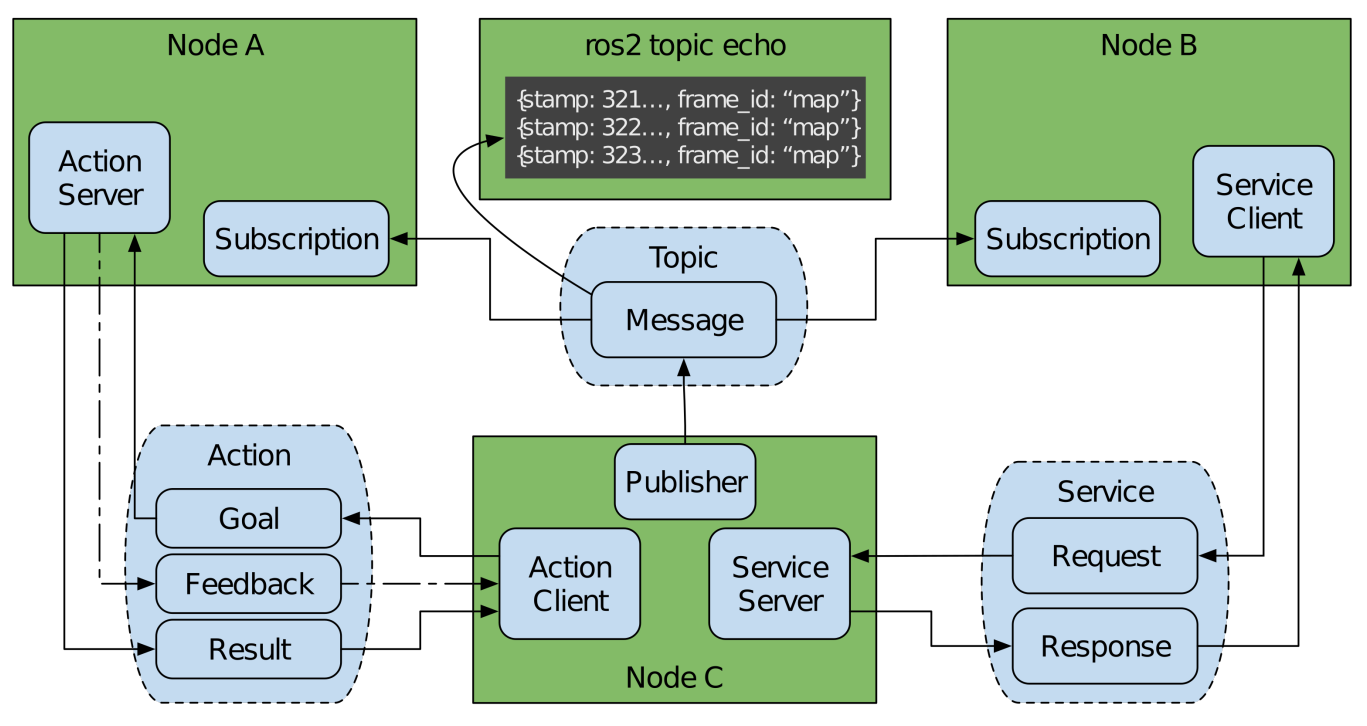
\includegraphics[width=\linewidth]{figures/background/ros2_node_interfaces.png}
    \caption[Communication patterns between \gls{ros}2 nodes]{Communication patterns between \gls{ros}2 nodes \cite{Macenski2022}}
    \label{fig:communication_patterns} 
\end{figure}

% Third paragraph introducing essential topics of ros1 and ros2
\gls{ros} provides a standardized abstraction of communication for robotic applications over multiple machines. This is ideal for use cases like cloud robotics and edge robotics. \gls{ros} provides three communication patterns: topics, services, and actions. A typical \gls{ros}2 application can be illustrated in \cref{fig:communication_patterns}. A \gls{ros} node is responsible for a single, module purpose, such as controlling the camera and doing image processing \cite{ROSGalactic2021} Each node can send and receive data to other nodes via the three communication patterns. The most common pattern is topics. The \gls{ros} nodes communicate by publishing and subscribing to messages on topics. Depending on what information needs to be communicated between the \gls{ros} nodes, the messages use the defined type. With the publish-subscribe pattern, the topics allow many-to-one, one-to-many. as well as many-to-many communication. The services provide a request-response communication. Clients submit requests to the service server, which processes the request and sends a response back to the client asynchronously. Actions provide goal-oriented and asynchronous communication interfaces with a request, response, and periodic feedback. This communication pattern is normally suitable for long-term complex tasks, such as navigation. Other than the communication patterns, the \gls{ros} node can also be configured via the \gls{ros} parameters at startup or during the runtime without changing the code. A \gls{ros} parameter usually needs to be first declared and then used somewhere in the \gls{ros} node. 

Since \gls{ros}2 galactic is the state-of-the-art during the work of this thesis, the name "\gls{ros}" refers to \gls{ros}2 galactic for the rest of the thesis unless specified otherwise. 

\subsection{Gazebo Simulation}

% First paragraph as an overview of Gazebo simulation

\gls{gazebo} is an open-source 3D simulator for robotics. It integrates a physics engine and a rendering engine, and support code for sensor simulation and actuator control \cite{GazeboWiki}. Therefore, the camera sensor can generate realistic RGB images from the simulation. The \gls{gazebo} simulation has undergone a series of name changes during its development, as shown in \cref{fig:gazebo_development}. The original \gls{gazebo}, also now known as \gls{gazebo} classic, is discontinued after the last generation released in 2020. The ignition name is initially used for another approach to differentiate itself from the original \gls{gazebo}, i.e., \gls{gazebo} classic, is changed back to \gls{gazebo} again in 2022 for the current state-of-the-art \gls{gazebo} garden. However, since this thesis uses Gazebo Fortress, due to dependency issues with \gls{ros}, the name \gls{gazebo} refers to \gls{gazebo} fortress for the rest of the thesis for simplicity. 

% Figure for gazebo development
\begin{figure}
    \centering
    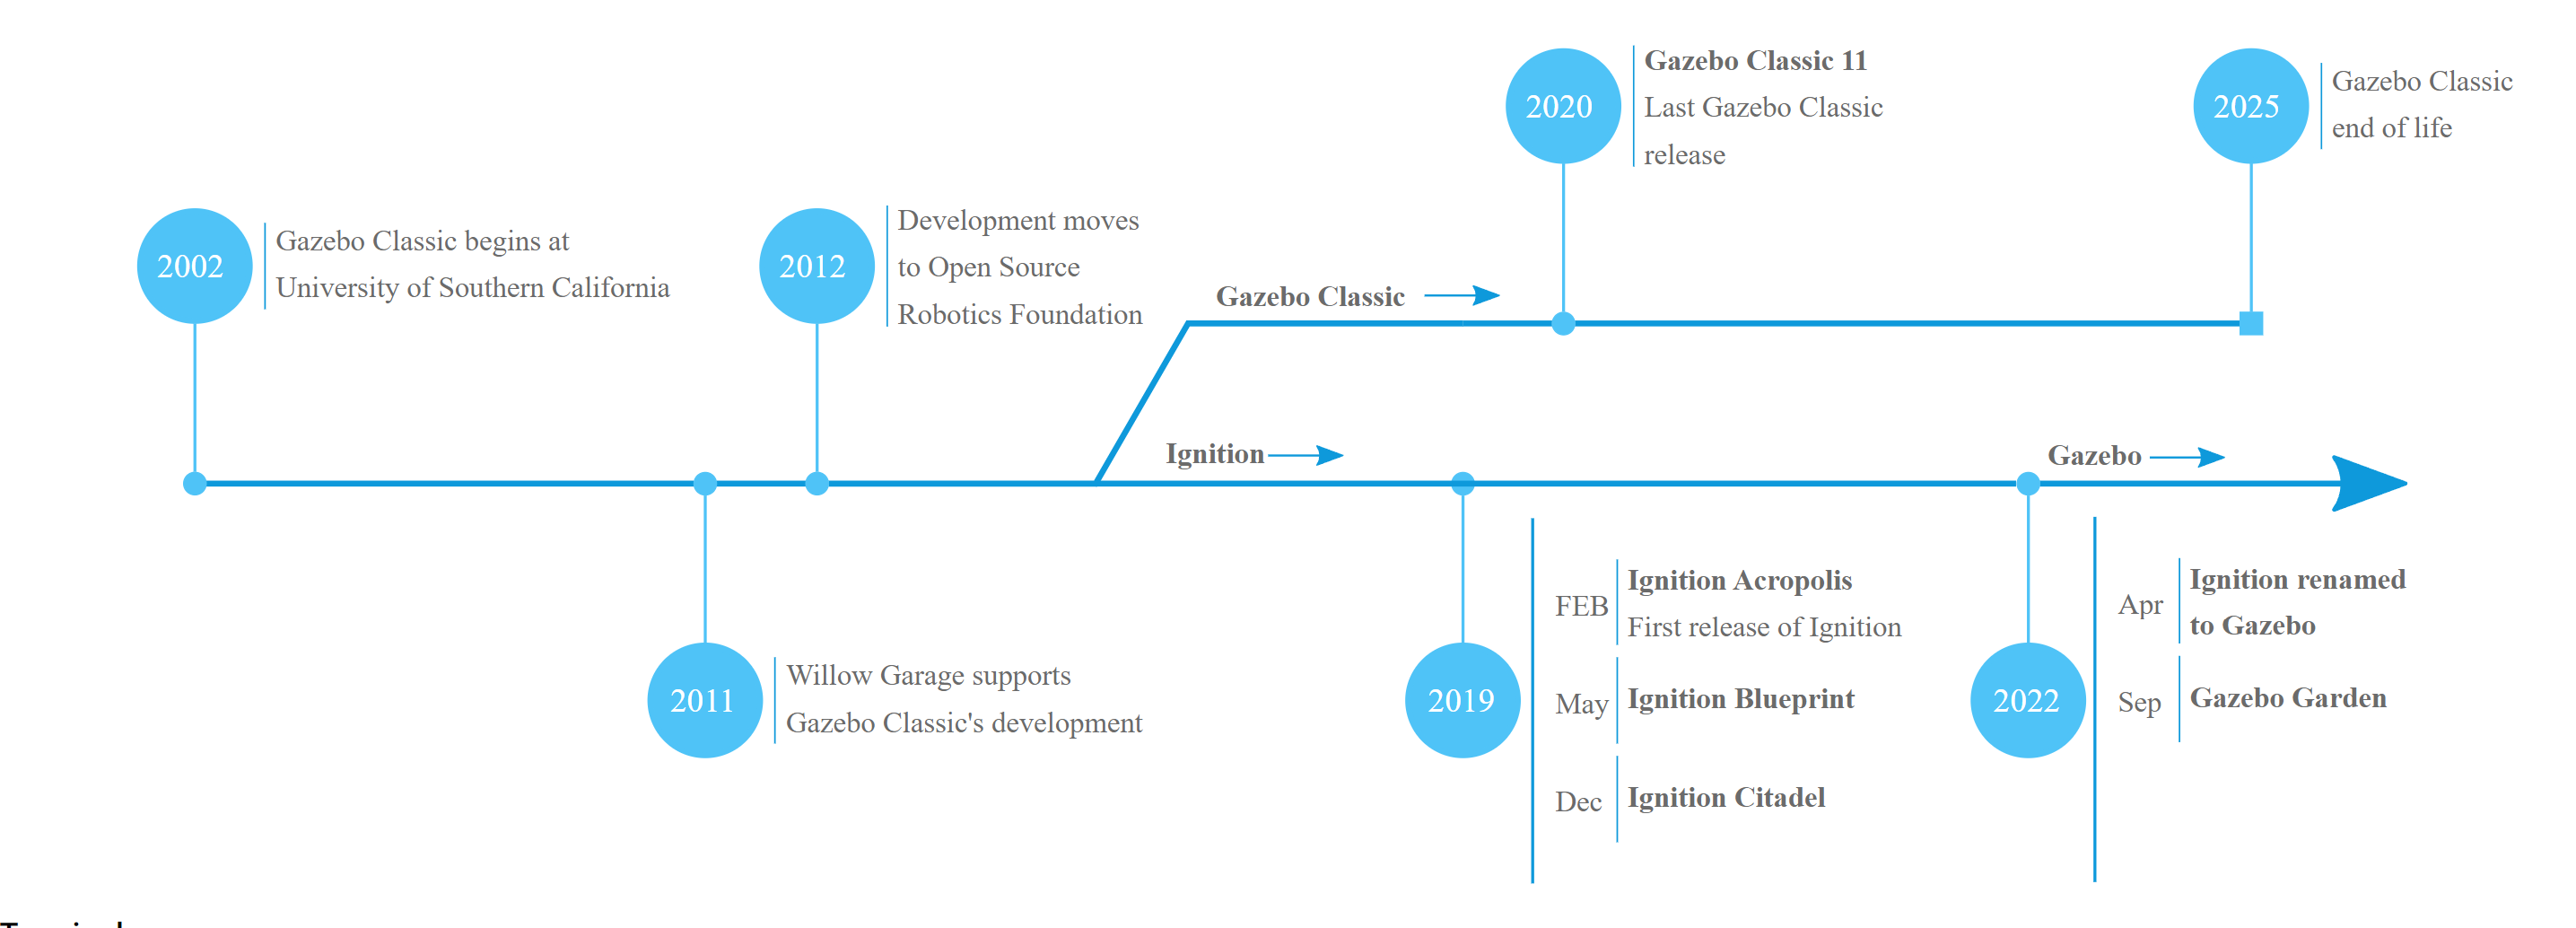
\includegraphics[width=\linewidth]{figures/background/gazebo_development.png}
    \caption{The development of \gls{gazebo} simulation \cite{GazeboSim}} 
    \label{fig:gazebo_development}
\end{figure}

In \gls{gazebo}, the simulation scenarios are implemented as world files and model files, which are written in \gls{sdf} \cite{SDFormat}. The \gls{gazebo} loads the world file on startup and it can load the model files either on startup or during runtime on demand. The \gls{gazebo} client runs a user interface for the server. Camera sensors and bounding box cameras sensors can generate RGB image stream and bounding boxes during simulations. The messages are published in protobuf format and they can be bridged to \gls{ros} messages with \gls{ros}-\gls{gazebo} bridge \cite{GazeboSim}. 

% Second paragraph introduce the development of Gazeob (Classic -> Ign -> Gz)

% Third paragraph introduce how a scenario is implemented in gazebo and what does the gazebo output

\subsection{Network policies}

\gls{netem} is an enhancement of the Linux traffic control facilities that allow one to add characteristics to packets outgoing from a selected network interface \cite{tc-netem}. It can add delay packet loss, duplication, as well as rate. An outgoing policy can be set up for network interface "eth0" as follows: 

\begin{verbatim}
    tc qdisc add dev eth0 root netem delay 100ms loss 10% rate 160Mbit
\end{verbatim}

In this example, the \gls{netem} set the outgoing policy of the network interface "eth0" to 100 ms delay, 10\% packet loss and 160 Mbps bandwidth. However, it is worth noticing that \gls{netem} can only set up outgoing policies. For incoming policies, a \gls{ifb} device needs to be set up and all traffic needs to be redirected to the new network interface. Then, the \gls{netem} can be used to modify the outgoing policies of the \gls{ifb} network interface, which will act as the incoming policies of the original network interface.
